\section{Related Work}
    
    \frame{\sectionpage}

    \begin{frame}{1/5 Success Rule}
        Adjust the mutation rate based on the success of recent generations. \begin{itemize}
            \item If success rate < 1/5, increase mutation rate (exploration).
            \item If success rate > 1/5, decrease mutation rate (exploitation).
            \item Otherwise, mutation rate remain unchanged.
        \end{itemize}
    \end{frame}
    
    \begin{frame}{Fitness Based}
        \begin{itemize}
            \item Change the mutation rate with current fitness and the average fitness by the ratio between them. \cite{Marsili_Libelli2000-tt}
            \item A local minima can be detected by the difference between population maximum fitness and average fitness. \cite{286385}
        \end{itemize}
        \centering
        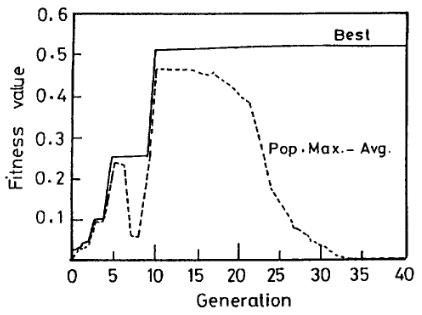
\includegraphics[height=0.5\textheight]{images/LocalOptimaDetection.png}
    \end{frame}

    \begin{frame}{Diversity Based}
        \begin{itemize}
            \item Monitoring and Adjustment
                \begin{itemize}
                    \item Measuring the population diversity using metrics like average distance\cite{fish,OSUNAENCISO2022192} or Shannon Entropy\cite{Stark2012ANS} .
                    \item If diversity drops, increase mutation rate to promote exploration and avoid stagnation.
                \end{itemize}
            \item Distance-Based Crossover Control
                \begin{itemize}
                    \item Often refer to Mating Distance \cite{eshelman1991preventing}.
                    \item Enforcing distance between parents.
                    \item By ensure the genetic difference to maintain population diversity.
                \end{itemize}
        \end{itemize}
    \end{frame}